\section{Case Study}
\label{sec:caseStudy}
To demonstrate the application of the hypervolume indicators and the proposed pairwise objective metric to the analysis of conflict in multi-objective systems, we perform a case study on forest management in the Deschutes National Forest. We compare the conflict among ecosystem services in three multi-objective systems: one in which climate change is ignored, one in which climate change is predicted to be mild, and one in which it is predicted to be severe. For each climate change scenario, we solve a multi-objective mathematical program that optimizes ecosystem service achievement. The model aims to minimize fire hazard and sediment delivery while maximizing habitat for the northern spotted owl. In the coming sections we describe the study area and the importance of each of these ecosystem services. We then formally define the mathematical program solved for each climate change scenario, describe the climate scenarios considered, and finally present and discuss the results.

\subsection{Study area and selection of ecosystem services}
\label{subsec:studyArea}
%To provide context for the selection of ecosystem services for the model, we first describe the area in which the case study was conducted.
Our study area is the Drink Planning Area. It consists of 7056 ha of federally owned forest land on the east slopes of the Cascade Mountain Range located within the Deschutes National Forest. See Figure \ref{fig:drinkOverview}. Having never undergone logging or treatment, the Drink contains large areas of old growth forest. The large swaths of old growth forest in the Drink make it prime habitat for the northern spotted owl (NSO) (\textit{Strix occidentalis caurina}, Figure \ref{fig:nso}), an iconic % (albeit controversial \cite{simberloff1998flagships}) 
inhabitant of Pacific Northwest forests that is listed as a federally threatened species \cite{congress1973endangered}. However, the same old growth conditions that render the area suitable habitat for the NSO also render it susceptible to high-severity wildfires. Such a wildfire would put at risk the NSO's habitat \cite{courtney2004scientific} as well as one of the Drink's other notable features - the municipal watershed for the cities of Bend, OR and Sisters, OR. Wildfires pose a threat to these cities' water supply, because they can cause soil water repellency, surface runoff, and debris torrents \cite{ice2004effects} which degrade watershed quality.

\begin{figure}[ht]
\centering
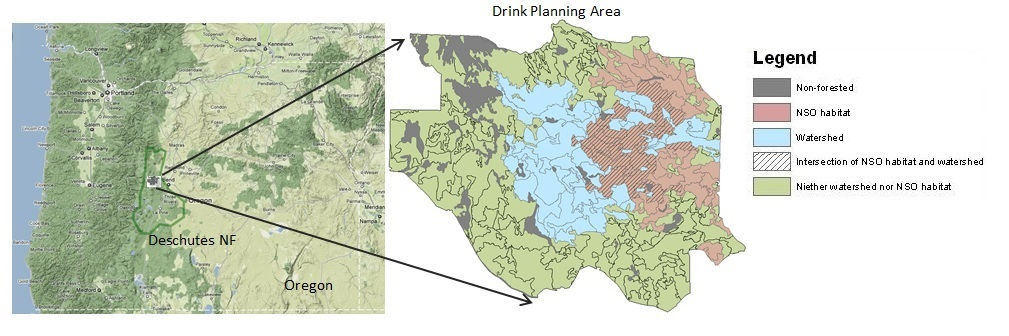
\includegraphics[width=.9\textwidth]{../images/Drink_Overview}
\caption[Overview of the study system, the Drink Planning Area]{Overview of the study system, the Drink Planning Area, consisting of 7056 ha in the Deschutes National Forest. The Drink Area contains old growth forest that make it suitable habitat for the northern spotted owl. It also houses the municipal watershed for Bend, OR and Sisters, OR.}
\label{fig:drinkOverview}
\end{figure}

\begin{figure}
\centering
\caption[Northern spotted owl]{The northern spotted owl is a threatened species whose habitat includes forests in the Pacific Northwest, including the Drink Area.}
\label{fig:nso}
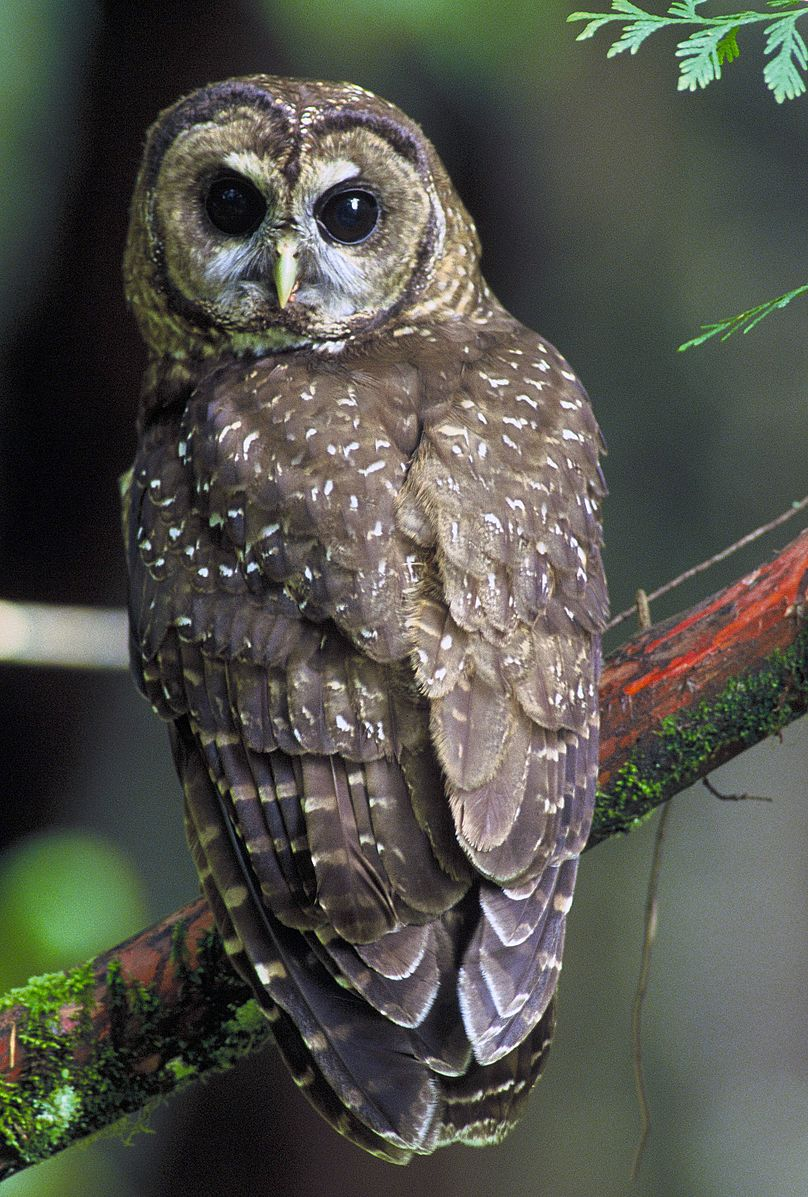
\includegraphics[width=.2\textwidth]{../images/NorthernSpottedOwl_USFWS}
\end{figure}

For these reasons, the managing entity, the United States Forest Service (USFS), would like to perform fuel removals in the Drink in order to reduce the area's fire hazard. However, performing these fuel removals has the potential to disrupt the habitat of the NSO \cite{bond2002short} and to induce short-term increases in sediment delivery \cite{o2005conceptual}. The latter is expected to be especially true in the Drink Area, where local USFS staff have noted that the watershed is unusually susceptible to spikes in sediment delivery as a result of foot traffic and other activities that occur within the watershed.

We developed a multi-objective mathematical program that optimizes the joint provision of these conflicting ecosystem services\footnote{These represent only a subset of the ecosystem services of concern to the USFS in the Drink Area. While the USFS manages for many ecosystem services simultaneously, many of the services are stacked rather than bundled, meaning the ecosystem services are not in conflict. These services need not all be considered in the multi-objective model, because the selection and maximization of one ecosystem service entails the maximization of all in the stack. For this reason, we have disregarded non-conflicting ecosystem services and selected a minimal bundle on which to employ multi-objective optimization. Those that do not conflict can be stacked post-optimization.}.

\subsection{The multi-objective model}
The multi-objective model is a zero-one mathematical program that assigns spatiotemporal prescriptions for fuel removals across the Drink Area to optimize the joint provision of ecosystem services. Spatially, the model prescribes fuel removals across 303 forest stands into which the Drink has been divided (the interior polygons in Figure \ref{fig:drinkOverview}). Temporally, the model operates over an 80-year planning horizon, from 2015 to 2095. The fuel removals are scheduled in two 20-year treatment periods: 2015-2035 and 2035-2055. For each stand, the model may prescribe fuel removals in the first period, the second period, neither, or both.

To ensure long-term efficacy of the fuel removals, the model minimizes the fire hazard rating of the Drink Area at the end of the 80-year planning horizon. To mitigate impacts of the fuel removals on NSO habitat, the model maximizes the area of NSO habitat at the end of each planning period. Similarly, the model minimizes the short-term spikes in sediment delivery resulting from the application of fuel removals, which are assumed to be performed at the midpoint year in the treatment periods (years 2025 and 2045). Figure \ref{fig:drinkPlanningHorizon} contains a schematic of the planning horizon which shows the timing of these events.

\begin{figure}
\centering
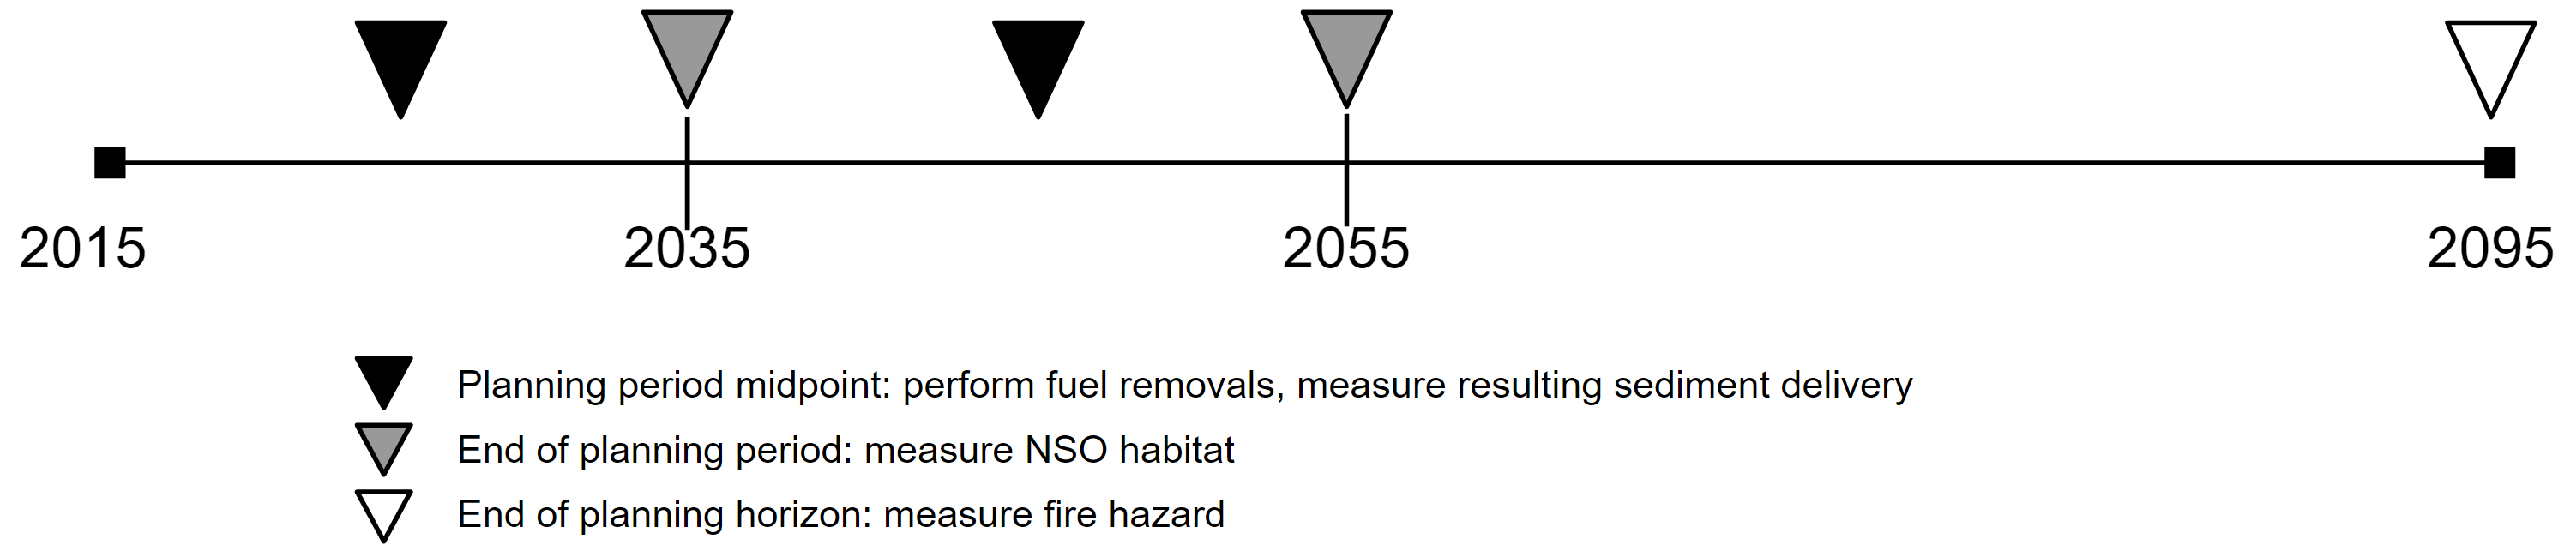
\includegraphics[width=.9\textwidth]{../images/Drink_PlanningHorizon_Sketch}
\caption[Planning horizon for the case study]{The planning horizon used in the case study spans the 80 year period from 2015 to 2095. Fuel removals may be performed in the first period (2015-2035), the second period (2035-2055), both, or neither. Fuel removals are assumed to be performed at the mid-point years of each period (black triangles). Sediment delivery is measured on treatment years. Stands' suitability for NSO habitat is measured at the end of the planning periods (gray triangles), and stands' fire hazard ratings are measured at the end of the planning horizon (white triangle).}
\label{fig:drinkPlanningHorizon}
\end{figure}

\subsubsection{Notation}
We use the following notation in the development of the model:

\paragraph{Model parameters}
\begin{itemize}
\item \textbf{$i \in I$:} the set of forest stands comprising the Drink Area ($|I| = 303$)

\item \textbf{$a_i$:} the area of stand $i$

\item \textbf{$r \in R$:} the set of fuel removal prescriptions:
	$$
	r =
	\begin{cases}
	1 &\text{ fuel removals in the first period (2015-2035)}\\
	2 &\text{ fuel removals in the second period (2035-2055)}\\
	3 &\text{ fuel removals in both periods}\\
	0 &\text{ no fuel removals performed in either period}
	\end{cases}
	$$
	
\item \textbf{$F_{i,r}$:} the area-weighted fire hazard rating of stand $i$ at the end of the planning horizon if prescribed to fuel removal schedule $r$. The metric for fire hazard rating used in this analysis originated in the work by Schroder \textit{et al.} \cite{schroder2016multi}. This metric was developed for the Drink Area. It uses fire characteristics from the set of fuel models proposed by Anderson \cite{anderson1982aids} in order to assign a fire hazard rating. I expanded the rating system to include fuel models not present in Schroder \textit{et al.} See Table \ref{tab:firehazards} for the mapping of fuel models to fire hazard ratings.

The USFS's Climate-Forest Vegetation Simulator (Climate-FVS) was used to generate the fuels and vegetation characteristics of the stands in order to determine their fire hazard rating. Initial vegetation data for Climate-FVS came from the 2012 GNN structure map (\url{http://lemma.forestry.oregonstate.edu/data/structure-maps}) from Oregon State University's Landscape Ecology, Modeling, Mapping \& Analysis (LEMMA) group. Plots from the LEMMA database were mapped to the stands in the Drink area in order to produce tree and stand lists. These lists were used with Climate-FVS to simulate the stands' vegetation and fuels characteristics forward for the duration of the planning horizon under each climate scenario. Input climate data for Climate-FVS was obtained through the Climate-FVS climate data server \cite{climateFVSReadyData}.

\begin{table}[!ht]
\centering
\resizebox{\textwidth}{!}{%
\begin{tabular}{l|c|crrr}
\multicolumn{1}{c|}{Fuel Model} & \multicolumn{1}{c|}{\textbf{Fire Hazard Rating}} & \multicolumn{1}{c}{Group} & \multicolumn{1}{c}{Flame length (m)} & \multicolumn{1}{c}{Rate of spread (m/hr)} & \multicolumn{1}{c}{Total fuel load (tons/ha)} \\ \hline
4*                              & \textbf{5}                                       & Shrub                     & 5.79                                 & 1508.76                                   & 32.12                                         \\
5                               & \textbf{4}                                       & Shrub                     & 1.22                                 & 362.10                                    & 8.65                                          \\
8                               & \textbf{1}                                       & Timber                    & 0.30                                 & 32.19                                     & 12.36                                         \\
9*                              & \textbf{2}                                       & Timber                    & 0.79                                 & 150.88                                    & 8.65                                          \\
10                              & \textbf{2}                                       & Timber                    & 1.46                                 & 158.92                                    & 29.65                                         \\
11*                             & \textbf{2}                                       & Logging Slash             & 1.07                                 & 120.7                                     & 28.42                                         \\
12                              & \textbf{4}                                       & Logging Slash             & 2.44                                 & 261.52                                    & 85.50                                         \\
13                              & \textbf{5}                                       & Logging Slash             & 3.20                                 & 271.58                                    & 143.57                                       
\end{tabular}%
}
\caption[Fire hazard ratings used in multi-objective model]{Fire hazard rating system used here, originally employed by Schroder \textit{et al.} \cite{schroder2016multi}.\\
Asterisks (*) denote fuel models not present in Schroder \textit{et al.}\\
The fuel model column refers to the Anderson fuel model ratings \cite{anderson1982aids}.}
\label{tab:firehazards}
\end{table}

\item \textbf{$I_{\omega,t}$:} the set of stands that qualify as NSO habitat at the end of planning period $t$ under at least one fuel removal schedule. The stands that qualify as NSO habitat at the end of a planning period $t$ are those that meet the following three criteria in year $t$, as specified by the USFS:
	\begin{enumerate}
	\item elevation less than 1830 m
	\item the presence of trees with diameter at breast height (DBH) at least 76 cm
	\item canopy closure of at least 60\%
	\end{enumerate}
The elevation requirement was checked using a digital elevation model from the US Department of Agriculture's GeoSpatial Data Gateway; canopy closure and large tree criteria were determined using the simulated vegetation characteristics output from Climate-FVS.

In addition, to account for the large habitat requirements of the NSO, stands must be members of a cluster exceeding 200 ha in size, the entirety of which meets the aforementioned NSO habitat criteria. Stands that meet the first three criteria but are not part of such a cluster are less valuable NSO habitat and therefore have their contributions to the total owl habitat discounted by a factor of $e$.

\item \textbf{$e$:} the discount factor applied to NSO habitat when it is not part of a contiguous habitat cluster at least 200 ha in size. Following the convention used in Schroder \textit{et al.} \cite{schroder2016multi}, we set $e = 0.5$.

\item \textbf{$j \in R_{i,t}$:} the set of fuel removal schedules such that stand $i$ qualifies as NSO habitat at the end of planning period $t$. For instance, consider stand $i=15$ and planning period $t=2$ (2035-2055). We seek to find the set of fuel removal prescriptions $r \in R$ such that stand 15 is suitable NSO habitat at the end of planning period 2 (in year 2055). We enumerate the vegetation characteristics of stand 15 for all possible fuel removal schedules and determine that if fuel removals are assigned in the second planning period, then stand 15 does not qualify as NSO habitat in year 2055. Thus, $R_{15,2} = \{0,1\}$, since for $r=0$ (no fuel removals performed) and $r=1$ (fuel removals performed in first period only), stand 15 does qualify as NSO habitat in 2055.

\item \textbf{$s_{i,t}$:} the amount of sediment (in tonnes) delivered to the watershed as a result of performing fuel removals on stand $i$ in planning period $t$. The contributions of sediment delivery from treatment of stand $i$ in period $t$ were determined using the online GIS tool for the Watershed Erosion Prediction Project (WEPP) \cite{frankenberger2011development}. This tool takes soil textures, treatment types, duration of simulation, and custom climate data as inputs. Soil texture data for the Drink area was obtained from the USDA's Soil Survey Geographic (SSURGO) database, treatment types are those specified in \S \ref{chap:appendix_drinkTreatments}, and the years of simulation correspond to the treatment years in the planning horizon (2015-2095). The custom climate data are those described above for use with Climate-FVS, obtained through the Climate-FVS data server.

\item \textbf{$c \in C$:} Recall that the quantification of NSO habitat depends on the availability of large contiguous habitat patches; areas of NSO habitat less than than 200 ha in size are discounted. In order to determine when habitat is provided in sufficiently large areas, we must enumerate the set of clusters of stands whose combined area exceeds 200 ha. This set of clusters is the set $C$.

\item \textbf{$i \in D_c$:} Given a cluster $c \in C$, the set $D_c$ is the set of stands that comprise cluster $c$.

\item \textbf{$c \in C_i$:} Given a stand $i$, we define the set $C_i$ as the set of clusters that contain stand $i$

\item \textbf{$A$:} the maximum area in hectares that may be treated in either planning period. We constrain the allowable treatment area per period to account for the limited availability of work crews to perform the fuel removals. Following guidance from the USFS, we set $A = 2428$ ha (approximately 6000 ac).

\item \textbf{$\ell$, $u$:} the lower and upper bounds, respectively, on the relative fluctuation in the area treated in periods 1 and 2. These bounds are used to enforce regulation in the workflow for the USFS. Here we use values such that the area for which fuel removals are performed does not fluctuate more than 20\% between treatment periods; that is, we set the lower bound $\ell = 0.8$ and the upper bound $u = 1.2$.
\end{itemize}

\paragraph{Decision Variables}
$$
x_{i,r} = \begin{cases}
1 &\text{ if stand $i$ is prescribed to treatment schedule $r$}\\
0 &\text{ otherwise}
\end{cases}
$$ 

\paragraph{Indicator Variables}
\begin{itemize}
\item \textbf{$q_{c,t} = 1$} if all stands in cluster $c$ qualify as NSO habitat at the end of planning period $t$; $q_{c,t} = 0$ otherwise
\item \textbf{$p_{i,t} = 1$} if in planning period $t$ stand $i$ is part of a cluster $c$ such that $q_{c,t} = 1$; $p_{i,t} = 0$ otherwise
\end{itemize}

\paragraph{Accounting Variables}
\begin{itemize}
\item \textbf{$S_t$:} the total sediment delivered to the watershed from performing fuel treatments in planning period $t$
\item \textbf{$O_t$:} the amount of NSO habitat (in hectares) at the end of planning period $t$
\item \textbf{$H_t$:} the total area (in hectares) treated in planning period $t$
\end{itemize}

\subsubsection{Model formulation}
The formulation of the multi-objective model is as follows:
\begin{align}
Minimize \quad & \notag\\
&\sum_{i\in I}\sum_{r\in R} F_{i,r} x_{i,r} \label{eqn:objFire} \\
&\max \{S_1,S_2\} \label{eqn:objSediment} \\
Maximize \quad & \notag\\
&\min \{O_1,O_2\} \label{eqn:objOwl}
\end{align}
Subject to:
\begin{align}
\sum_{i\in I_{\omega,t}} \left(a_i p_{i,t} + e a_i \left( \sum_{j \in R_{i,t}} x_{i,j}-p_{i,t} \right) \right) &= O_t \qquad \forall t \in \{1,2\} \label{eqn:constraintDefOwl}\\
\sum_{i\in I} \sum_{r\in 1,3} s_{i,1} x_{i,r} &= S_1 \label{eqn:constraintSediment1} \\
\sum_{i\in I} \sum_{r\in 2,3} s_{i,2} x_{i,r} &= S_2 \label{eqn:constraintSediment2} \\
\sum_{i \in D_c} \sum_{j \in R_{i,t}} x_{i,j} - |c| q_{c,t} &\ge 0 \qquad \forall t \in \{1,2\}, c \in C \label{eqn:constraintClusterTriggers} \\
\sum_{c \in C_i} q_{c,t} - p_{i,t} &\ge 0 \qquad \forall t \in \{1,2\}, i \in I_{\omega,t} \label{eqn:constraintPVarTriggers} \\
\sum_{r \in R} x_{i,r} &= 1  \qquad \forall i \in I \label{eqn:constraintOnePrescrip} \\
\sum_{i \in I} \sum_{r \in 1,3} a_i x_{i,r} &= H_1 \label{eqn:constraintAreaAcctg1} \\
\sum_{i \in I} \sum_{r \in 2,3} a_i x_{i,r} &= H_2 \label{eqn:constraintAreaAcctg2} \\
H_t &\le A \qquad \forall t \in \{1,2\} \label{eqn:constraintAreaRestr} \\
\ell H_1 - H_2 &\le 0 \label{eqn:constraintAreaFlucL} \\
-u H_1 + H_2 &\le 0 \label{eqn:constraintAreaFlucU} \\
x_{i,r}, p_i, q_c \in \{0,1\} \quad &\forall i \in I, r \in R, c \in C \label{eqn:constraintNonNeg}
\end{align}

Equations \eqref{eqn:objFire}-\eqref{eqn:objOwl} are the objective functions: equation \eqref{eqn:objFire} minimizes the cumulative fire hazard rating of the Drink Area at the end of the 80-year planning horizon, equation \eqref{eqn:objSediment} minimizes the maximum peak in sediment delivery for the two planning periods, and equation \eqref{eqn:objOwl} maximizes the minimum NSO habitat available at the end of the planning periods. Equation set \eqref{eqn:constraintDefOwl} defines the amount of NSO habitat available at the end of the planning horizons. Note that if stand $i$ does not belong to a cluster of NSO habitat exceeding 200 hectares, then its area contribution to total NSO habitat is discounted by a factor of $e$. Equations \eqref{eqn:constraintSediment1} and \eqref{eqn:constraintSediment2} define the sediment delivered in planning periods one and two, respectively.

Inequality set \eqref{eqn:constraintClusterTriggers} controls the value of the cluster variables $q_{c,t}$ indicating clusters that meet the NSO habitat criteria in each of the planning periods. Inequality set \eqref{eqn:constraintPVarTriggers} controls the value of the $p_{i,t}$ variables indicating whether stand $i$ is included in a cluster of NSO habitat at time $t$.

The set of equalities \eqref{eqn:constraintOnePrescrip} enforces the logical constraint that each stand must be prescribed to exactly one fuel removal schedule. Equations \eqref{eqn:constraintAreaAcctg1} and \eqref{eqn:constraintAreaAcctg2} are accounting constraints for the total area treated in each planning period, and inequalities \eqref{eqn:constraintAreaRestr} ensure that this area does not exceed the predefined maximum. Inequalities \eqref{eqn:constraintAreaFlucL} and \eqref{eqn:constraintAreaFlucU} bound the fluctuation in treated area between the planning periods. Finally, constraint \eqref{eqn:constraintNonNeg} defines the decision and indicator variables as binary.

\subsection{Solution method}
We developed an implementation of T\'{o}th's Alpha-Delta algorithm \cite{TothThesis} to solve the model \eqref{eqn:objFire}-\eqref{eqn:constraintNonNeg} utilizing the IBM ILOG CPLEX optimization engine. For a problem with $M$ objectives, the Alpha-Delta algorithm finds the Pareto frontier by iteratively slicing the $M$-dimensional objective space with a tilted $M-1$-dimensional hyperplane. The algorithm was implemented using an alpha parameter of $\alpha = .01$ and delta parameters of $\delta_{Hab} = 1$ ha and $\delta_{Sed} = 2$ tonnes for the NSO habitat and sediment delivery objectives, respectively.

\subsection{Climate change scenarios}
\label{sec:climateChange}
Like other ecosystems, forests will undergo changes as a result of the changing climate. For instance, researchers anticipate new spatial distributions of tree species \cite{iverson1998predicting}, increased sediment delivery to streams \cite{Goode20121}, and increasing disturbance regimes such as wildfires, droughts, and insect infestations \cite{vose2012effects}. As these transformations occur, the ability of forests to provide ecosystem services will change.

The extent of change will likely depend on the severity of the realized climate change. Thus, to understand the potential impacts on ecosystem services, multiple climate change scenarios representing a range of severities should be considered. We use three in our case study: one scenario in which climate change is ignored, ``None''; one in which climate change is predicted to be mild, ``Ensemble RCP 4.5'' (also ``E45''); and one in which climate change is predicted to be severe, ``Ensemble RCP 8.5'' (also ``E85''). These scenarios differ in their assumption of the additional energy per unit area that will be absorbed by the atmosphere, a value known as radiative forcing (RF). E45 assumes an RF of 4.5 $W/m^2$ and E85 assumes 8.5 $W/m^2$. In general, larger values of RF correspond to more severe climate change.

A given value of radiative forcing does not map to a single prediction of climate change, because researchers may disagree in how the climate will respond to that amount of RF. This is why for a given RF numerous climate models exist. A common approach to handling the disagreement among the climate models is to use an ensemble of climate models that all assume the same RF. We adopt this approach here for our E45 and E85 scenarios.

Each of these scenarios corresponds to an ensemble of 17 climate models. These climate models originate from the Fifth Assessment (AR5) on climate performed by the Intergovernmental Panel on Climate Change (IPCC). The selection and assembly of the 17 climate models used in these ensembles was conducted by Cookston (2016) and the Climate-FVS team \cite{ClimateModelsInFVSEnsemble}.

The other scenario, None, ignores any effects of climate change. While the number of studies incorporating climate change is increasing, this is still a common assumption in modern studies such as Schroder \textit{et al}. (2013) \cite{schroder2016multi}. Because it has served as the basis for many past studies of ecosystem services, the None climate scenario serves as a control against which we will compare the other two.

Each climate scenario corresponds to a different parameterization of the model, since the vegetation, fuels, and sediment delivery data depend on climate. Thus, changing the climate scenario has the potential to affect the amount and location of NSO habitat, the effects of fuel removals on NSO habitat, the fire hazard of the Drink Area, the efficacy of the fuel removals in reducing fire hazard, and the sediment delivered as a result of fuel removals. This drives changes to the relationships among the ecosystem services as well, which we investigate using the aforementioned conflict measures.


\subsection{Results}
We parameterized and solved the multi-objective model (\eqref{eqn:objFire}-\eqref{eqn:constraintNonNeg}) for each of the climate scenarios, generating three efficient frontiers: $Z_{\text{None}}$, $Z_{E45}$, and $Z_{E85}$ for the None, Ensemble RCP 4.5, and Ensemble RCP 8.5 scenarios, respectively. Figure \ref{fig:frontiersAll} shows the frontiers in their 3-dimensional objective spaces while Figure \ref{fig:frontiersPCPlot} provides a parallel coordinates view of the frontiers. The summary details of their objective achievements are listed in Table \ref{tab:frontiersSummary}.

\begin{table}[]
\centering
\caption[Summary of objective achievement across climate scenarios]{Summary of the performance of the efficient frontiers for each climate change scenario.}
\label{tab:frontiersSummary}
\begin{tabular}{lllll}
\multicolumn{2}{l|}{}                                                  & \textbf{None} & \textbf{E45} & \textbf{E85} \\ \hline
\multirow{3}{*}{\textbf{Fire hazard}}       & \multicolumn{1}{l|}{min} & 21321.21      & 23219.82     & 23268.02     \\
                                            & \multicolumn{1}{l|}{avg} & 21406.26      & 23324.41     & 23369.57     \\
                                            & \multicolumn{1}{l|}{max} & 21933.29      & 23973.79     & 23724.98     \\ \hline
\multirow{3}{*}{\textbf{NSO habitat}}       & \multicolumn{1}{l|}{min} & 2532.33       & 2412.18      & 2171.10      \\
                                            & \multicolumn{1}{l|}{avg} & 2536.31       & 2447.92      & 2421.99      \\
                                            & \multicolumn{1}{l|}{max} & 2540.05       & 2477.18      & 2481.01      \\ \hline
\multirow{3}{*}{\textbf{Sediment delivery}} & \multicolumn{1}{l|}{min} & 0             & 0            & 0            \\
                                            & \multicolumn{1}{l|}{avg} & 10.25         & 27.98        & 31.19        \\
                                            & \multicolumn{1}{l|}{max} & 24.57         & 63.43        & 69.68        
\end{tabular}
\end{table}


\begin{figure}[ht!]
  \subfloat[None]{%
    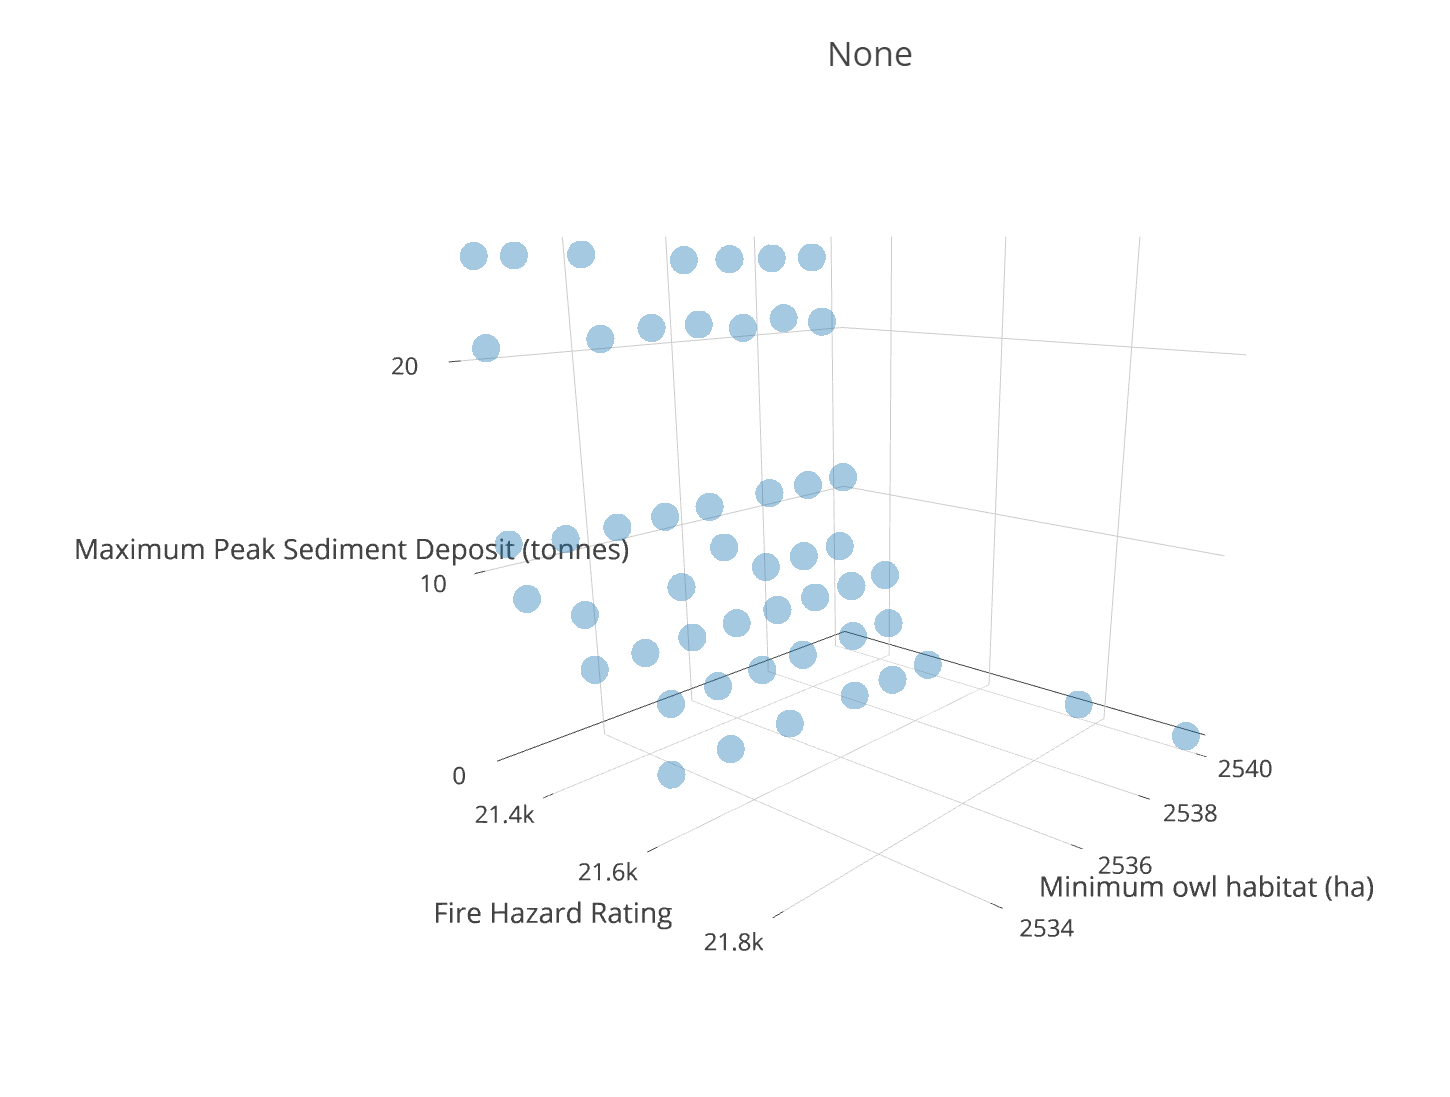
\includegraphics[width=.49\textwidth]{../images/Frontier_None}%
    \label{fig:frontierNone}%
  }
  \subfloat[Ensemble RCP 4.5]{%
    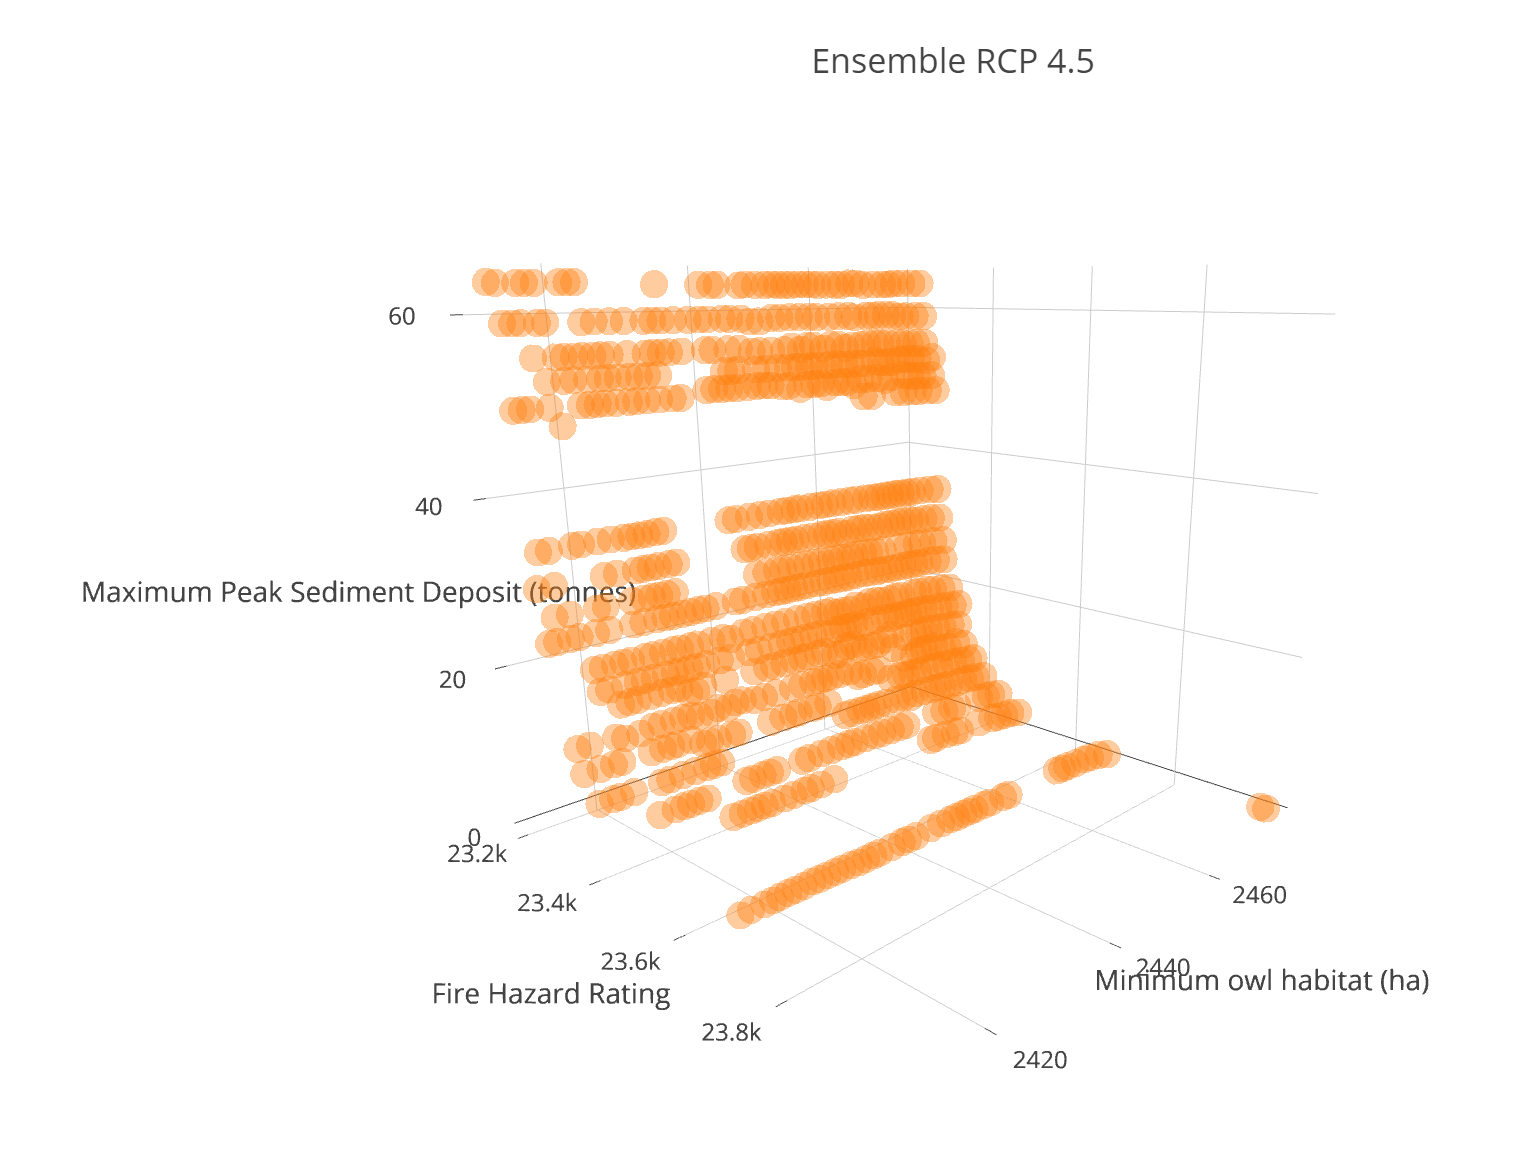
\includegraphics[width=.49\textwidth]{../images/Frontier_E45}%
    \label{fig:frontierE45}%
  }\hfill\centering
  \subfloat[Ensemble RCP 8.5]{%
    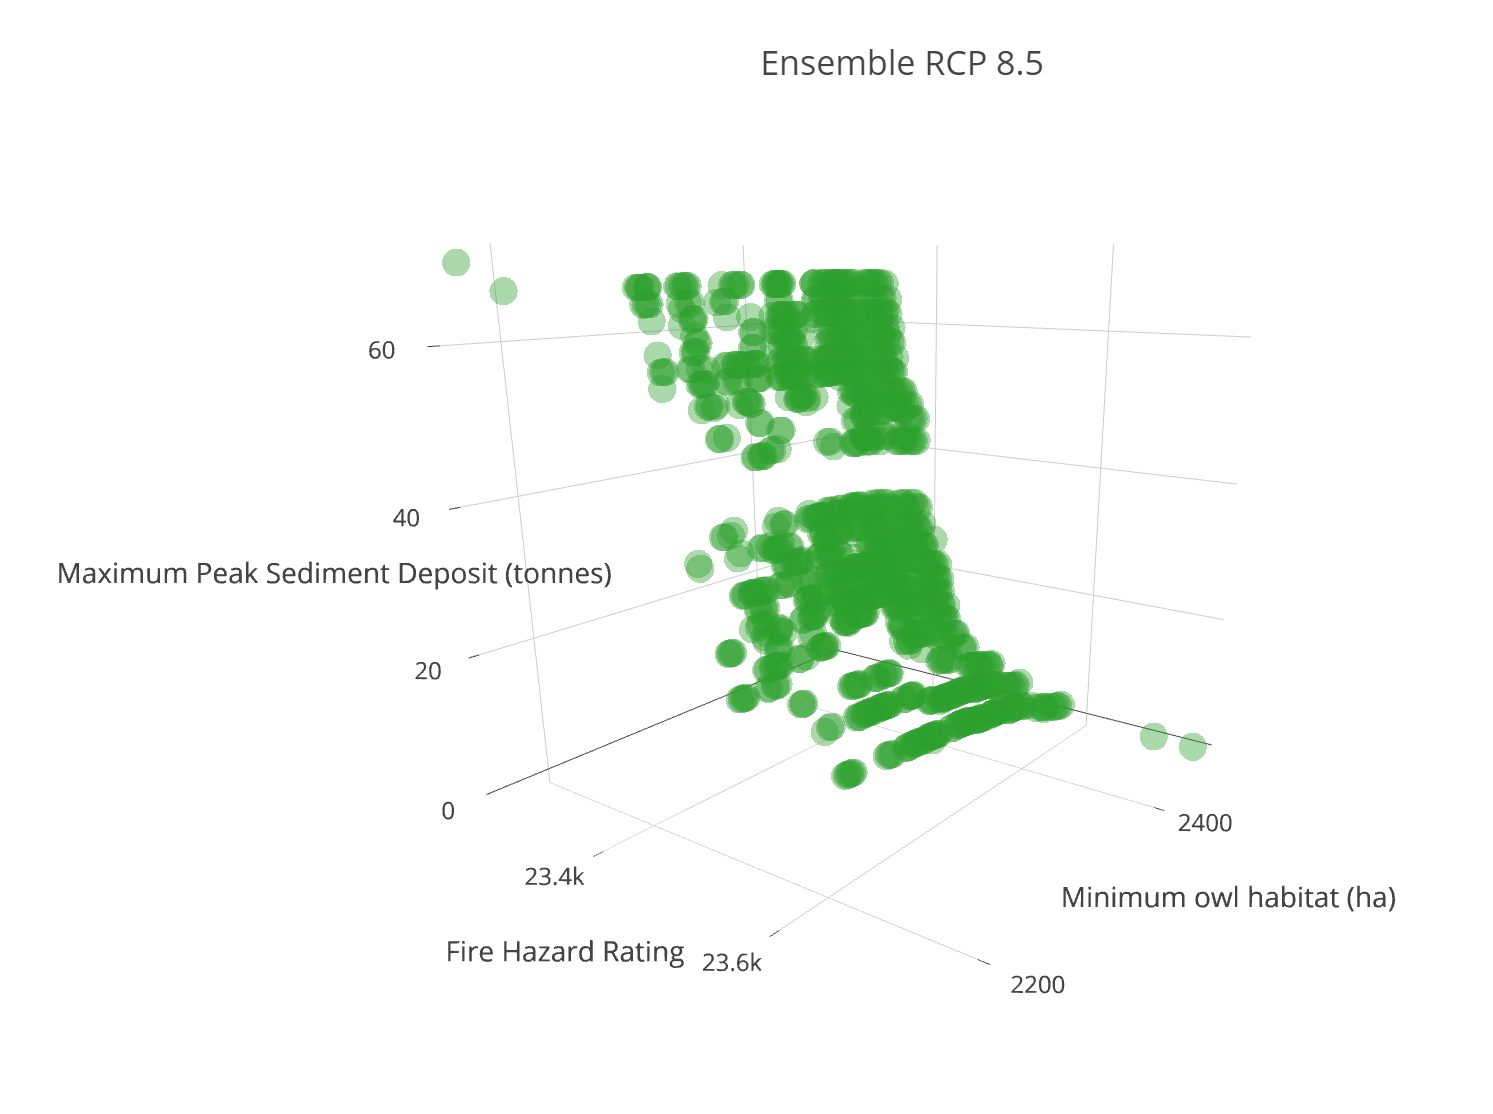
\includegraphics[width=.49\textwidth]{../images/Frontier_E85}%
    \label{fig:frontierE85}%
  }
  \caption[Frontiers for each climate change scenario]{Efficient frontiers for each climate change scenario.}
  \label{fig:frontiersAll}
\end{figure}

\begin{figure}[ht]
\centering
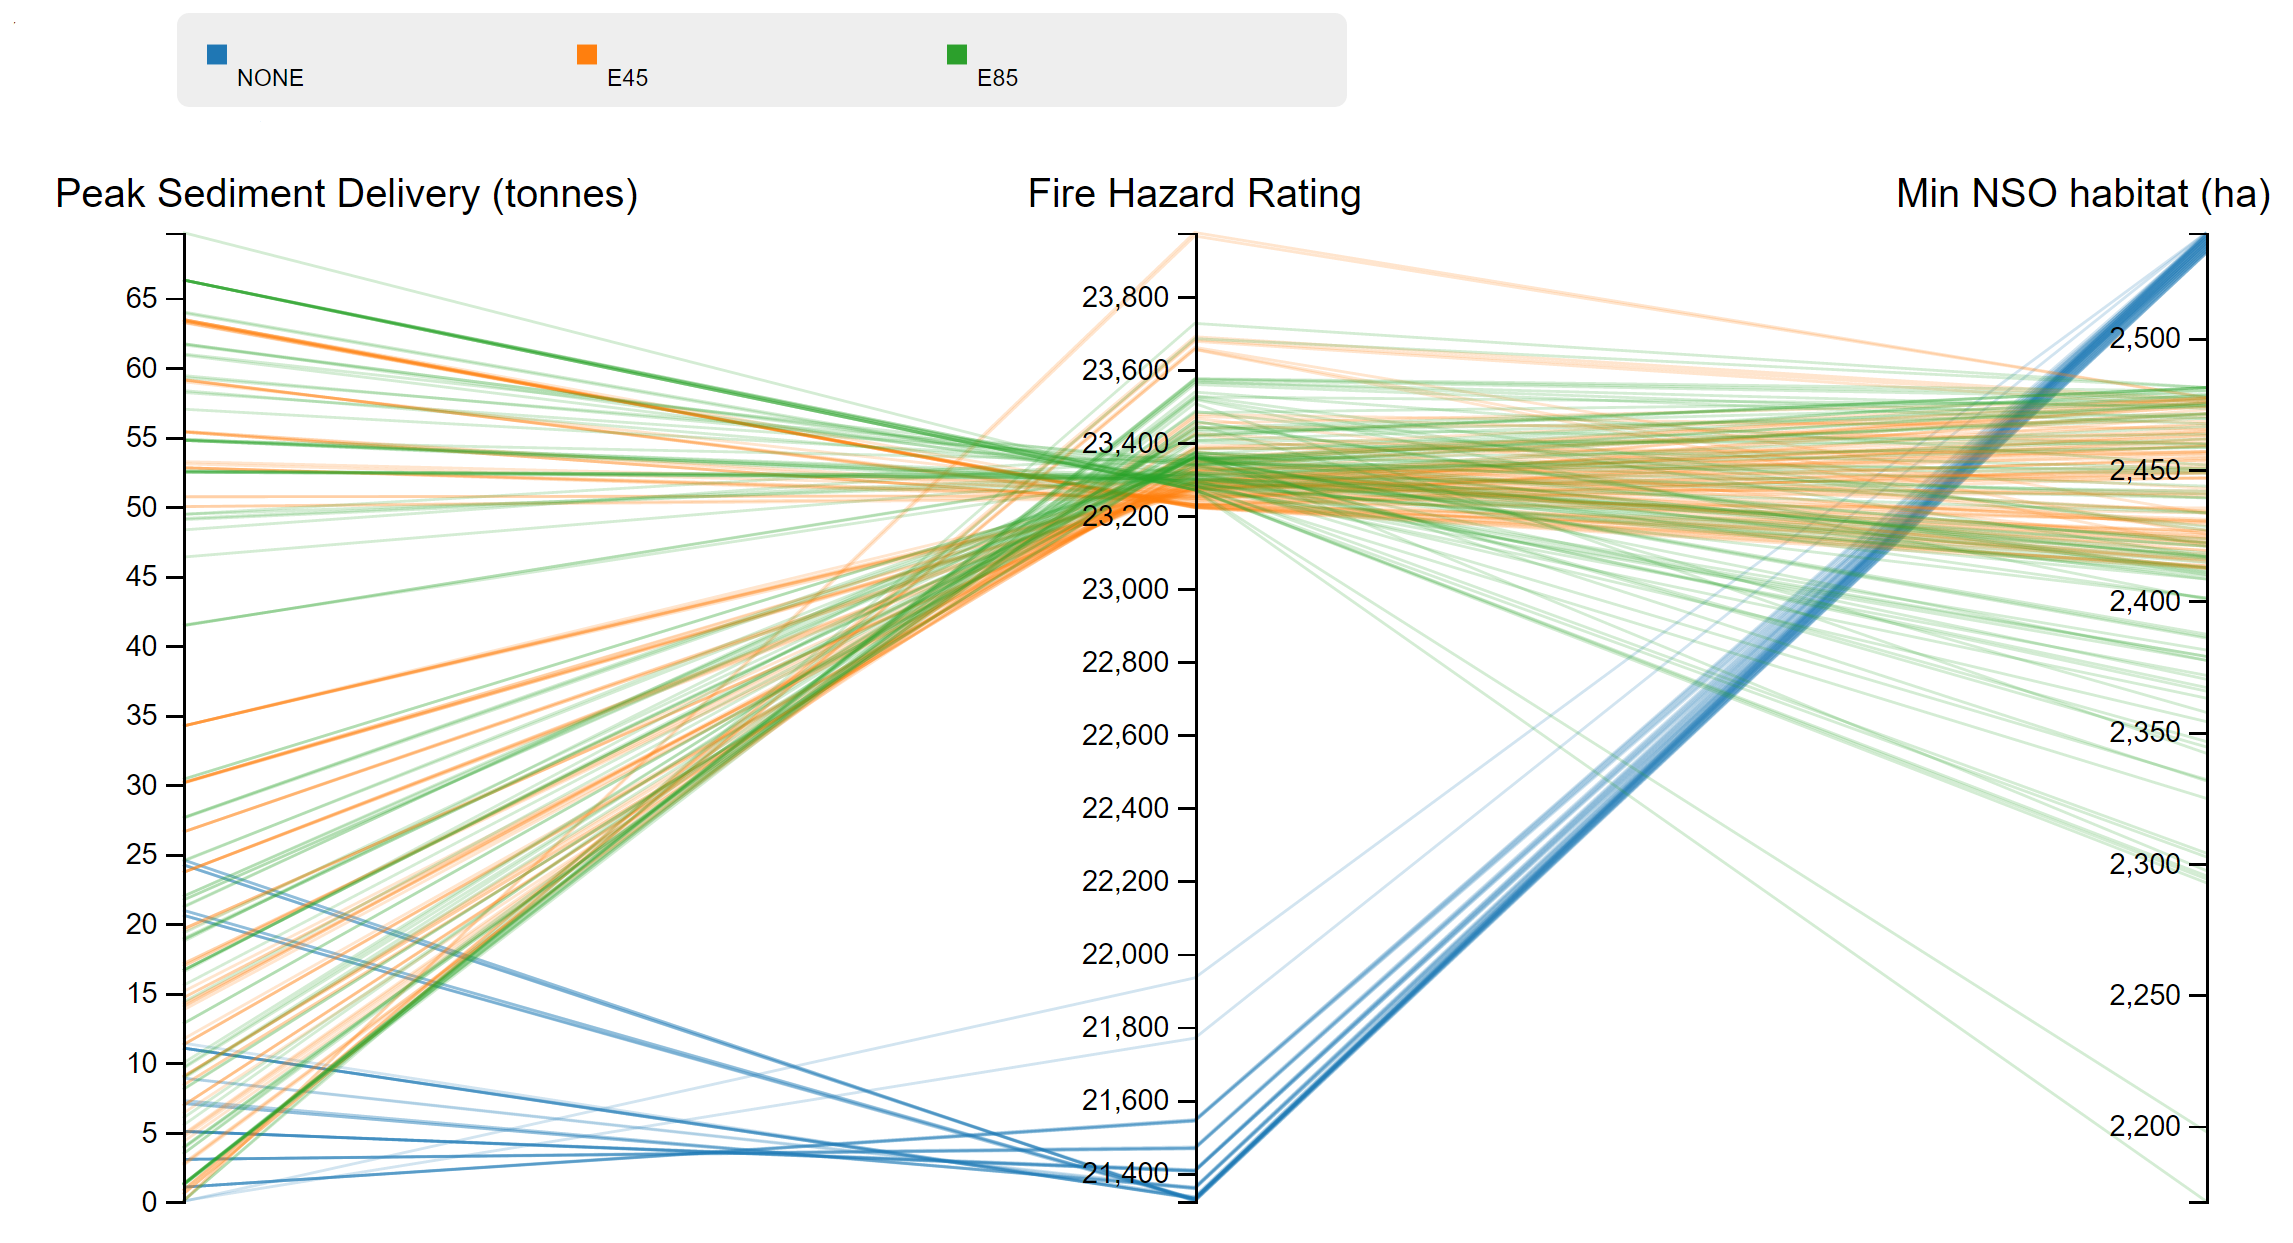
\includegraphics[width=.85\textwidth]{../images/FrontiersPCPlot}
\caption[Parallel coordinates view of the three frontiers]{Parallel coordinates view of the frontiers. Each axis represents an ecosystem service optimized by the model and each line a solution. In all objectives, we notice that None appears to outperform both the E45 and E85 scenarios, which show similar average objective achievements. To increase visual clarity, only a subset of solutions for E45 and E85 are shown because of the number of solutions in these frontiers.}
\label{fig:frontiersPCPlot}
\end{figure}

We first report the impacts of climate change on the provision of individual ecosystem services before analyzing its impacts on the joint provision of ecosystem services and the conflict among them.

\subsubsection{Individual provision of ecosystem services}
The average achievement of all ecosystem services decreases with increasing severity of climate change (see Table \ref{tab:frontiersSummary}, ``avg'' rows). We find that the difference in ecosystem service provision is greater between the assumption of no climate change and mild climate change (None to E45) than it is between mild climate change and severe climate change (E45 to E85).
%BEGIN DISCUSSION
This suggests that, for the ecosystem services in this study, the realization of climate change is more significant than the severity of that change. The model data provide evidence of why this is the case.

\paragraph{Sediment delivery} 
Compared to the None scenario, the average amount of sediment delivered is 172\% higher in E45 and 204\% higher in E85.
%BEGIN DISCUSSION
To understand why this may be, consider Figure \ref{fig:avgSedimentDelivery}. The figure shows the average tonnes of sediment delivered as a result of performing fuel removals for each climate change scenario. The sediment delivery per fuel removal under E45 is nearly twice the sediment delivery under the None scenario (81\% higher), whereas the E85 scenario is only 0.4\% higher than the E45 scenario.

% BEGIN DISCUSSION
This is a result of the response in sediment delivery to prescribed burns and the frequency with which they are assigned\footnote{For additional information on how stands are assigned a specific fuel removal technique such as thinning or prescribed burn, see the appendix, \S \ref{chap:appendix_drinkTreatments}.}. Our simulations show that increasing the severity of climate change causes pronounced increases in sediment delivery as a result of prescribed burns. We also find that relative to the None scenario, prescribed burns are assigned more frequently in the climate change scenarios: 8 times more frequently in E45 and 10.1 times more frequently in E85. See Table \ref{tab:prscBurnsInClimChange}. These effects combine to produce the result seen in Figure \ref{fig:avgSedimentDelivery} of increasing sediment levels with climate change severity.

\begin{figure}[ht]
\centering
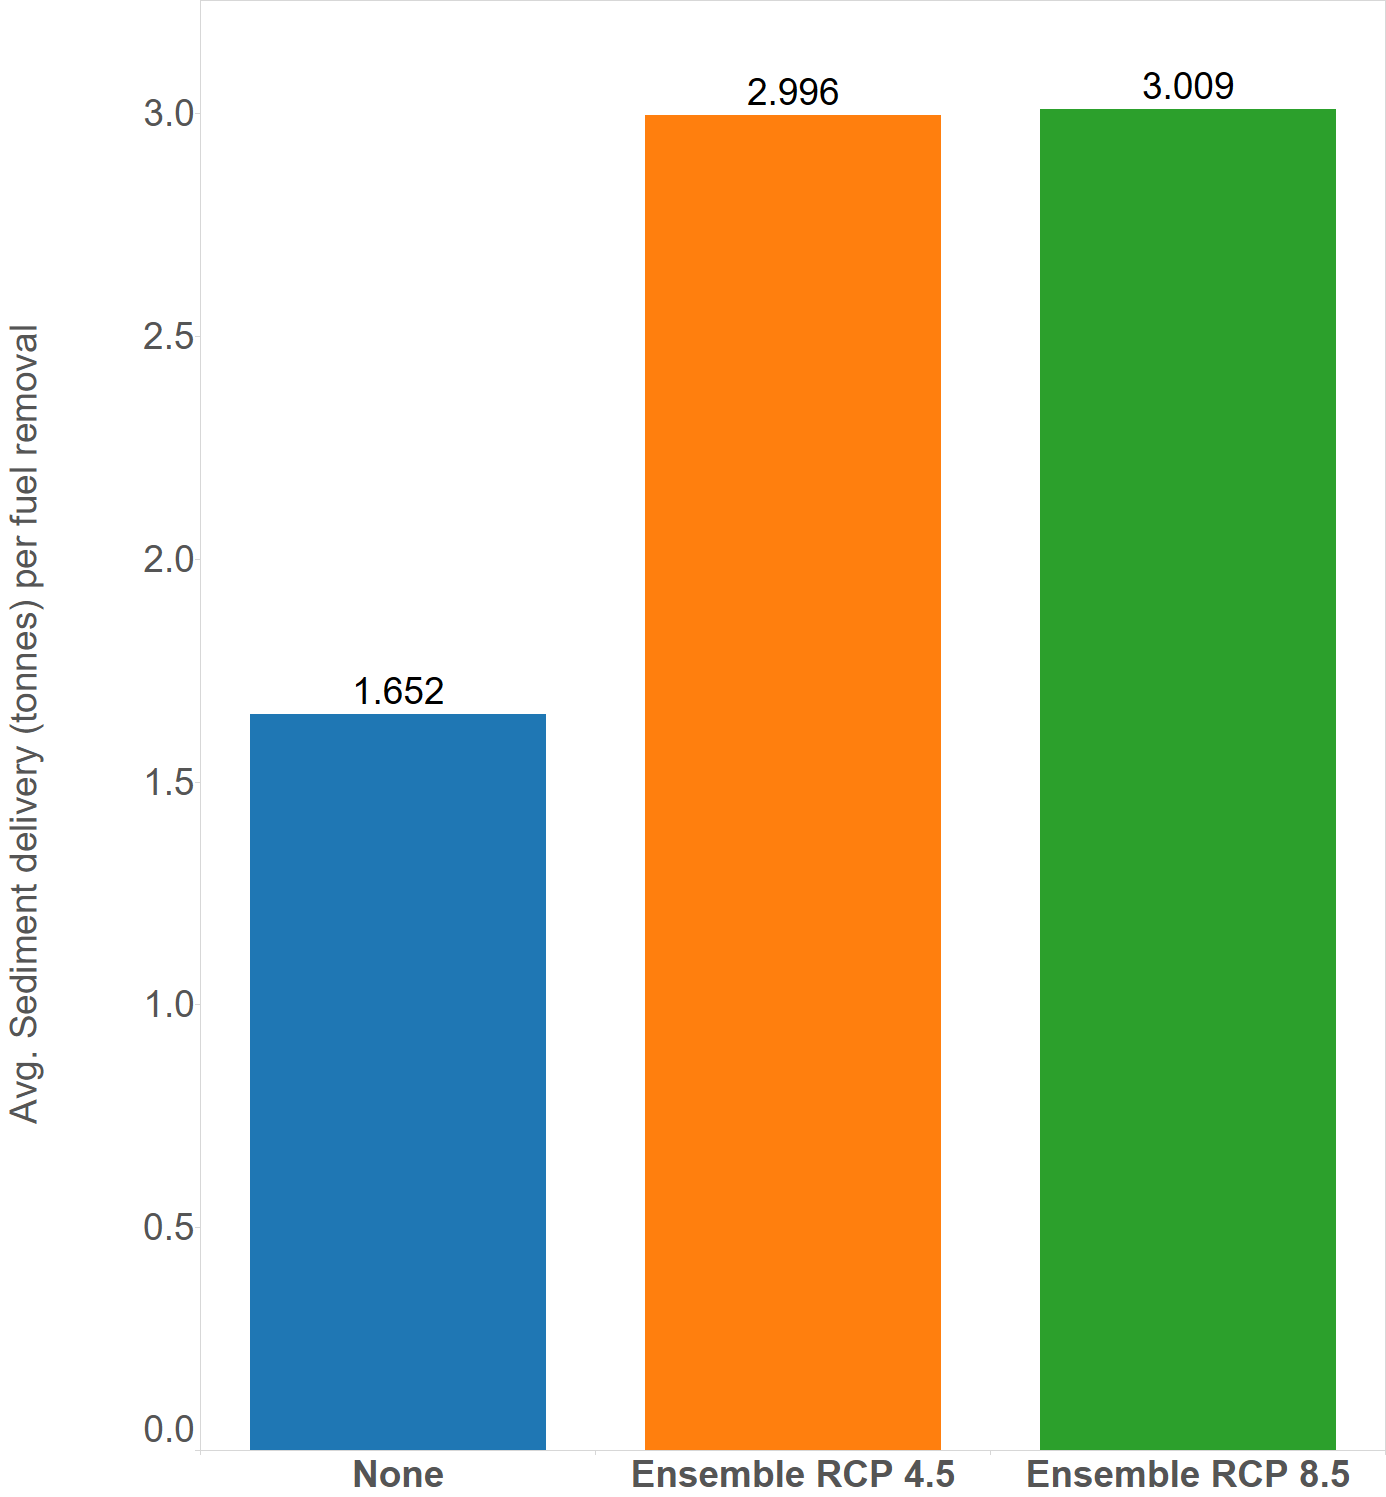
\includegraphics[width=.55\textwidth]{../images/AvgSedimentSpikes}
\caption[Average sediment delivery across climate scenarios]{Average spike in sediment delivery as a result of performing fuel removals for each of the climate change scenarios.}
\label{fig:avgSedimentDelivery}
\end{figure}

\begin{table}[]
\centering
\caption[Frequency and impact of prescribed burns across climate scenarios]{Frequency and impact of prescribed burn for each climate scenario. The combination of more frequent prescribed burns and increased sediment delivery per prescribed burn results in the higher values of sediment delivery in E45 and E85 observed in Figure \ref{fig:avgSedimentDelivery}.}
\label{tab:prscBurnsInClimChange}
\begin{tabular}{l|lll}
                                                                                                           & \textbf{None} & \textbf{E45} & \textbf{E85} \\ \hline
\textbf{\begin{tabular}[c]{@{}l@{}}Average sediment delivery\\ (tonnes) from prescribed burn\end{tabular}} & 31.23            & 48.56          & 48.97          \\
\textbf{\begin{tabular}[c]{@{}l@{}}Number of prescribed\\ burns assigned\end{tabular}}                     & 34         & 272        & 344       
\end{tabular}
\end{table}

\paragraph{Fire hazard}
Similarly, we find that the average fire hazard of the Drink Area increases with climate change severity, with E45 and E85 both performing approximately 9\% worse than None.
% BEGIN DISCUSSION
First, we note that this is not due to the model simply selecting less area for treatment under the climate change scenarios, as this value is essentially constant across both treatment periods and all climate scenarios (see Table \ref{tab:treatedAreas}). Instead, we find that the increase in fire hazard is due to the impact of climate change on the fuel model classification of the stands in the Drink Area. In E45 and E85, more stands are assigned a fuel model classification that is associated with higher fire hazard (refer to table \ref{tab:firehazards} for the mapping from fuel model to fire hazard). This is shown in Figure \ref{fig:distOfFireHazards}, where we observe a larger percentage of stands having a fire hazard rating of either 4 or 5 under the E45 and E85 scenarios than in None.

\begin{table}[]
\centering
\caption[Area treated per period across climate scenarios]{Areas treated per period across climate scenarios. The values are nearly the same for both periods and for each climate scenario.}
\label{tab:treatedAreas}
\begin{tabular}{l|lll}
                                                                                                           & \textbf{None} & \textbf{E45} & \textbf{E85} \\ \hline
\textbf{Area treated (ha) in period 1} & 2427.31            & 2426.90 & 2414.58          \\
\textbf{Area treated (ha) in period 2}                     & 2427.56         & 2427.71        & 2427.63      
\end{tabular}
\end{table}

\begin{figure}[ht]
\centering
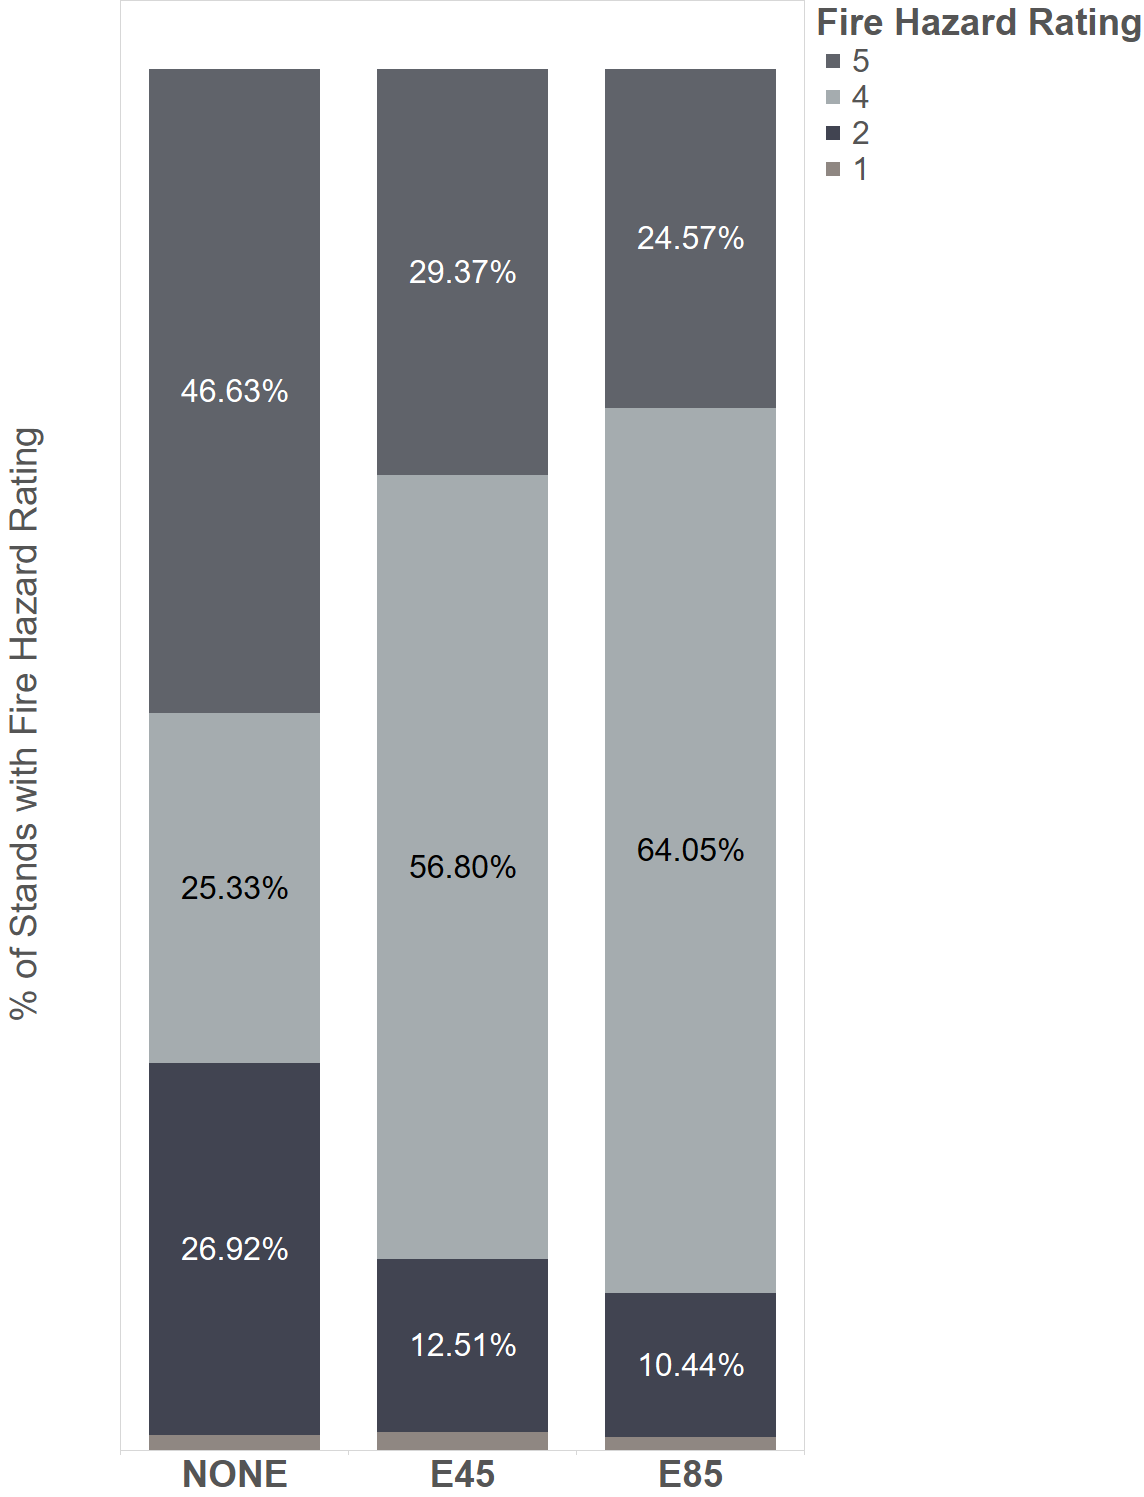
\includegraphics[width=.5\textwidth]{../images/FireHazardRatingsPerClimateScenario}
\caption[Distribution of fire hazard ratings over the Drink Area for each climate change scenario]{Distributions of fire hazard ratings across the Drink Area under each climate change scenario. Moving from left to right (in increasing climate change severity), we observe an increase in the number of stands classified with more extreme fire hazards (ratings of 4 and 5).}
\label{fig:distOfFireHazards}
\end{figure}
% If we need a map, show a single map that shows the diff in FH at 2095 for a good sol from E85 - good sol from None

\paragraph{NSO habitat}
Finally, we also observe a decrease in the average provision of NSO habitat under the consideration of climate change. The average provision in the E45 scenario is 88.4 ha less than in None, and E85 is 114.3 ha less.
% BEGIN DISCUSSION
The result is largely due to the effects of climate change on the vegetation characteristics that define whether a stand qualifies as NSO habitat. Of the criteria used, two of them are determined by vegetation characteristics: the presence of at least one tree with DBH $> 76$ cm and canopy closure of at least 60\%. While climate change has minimal impact on the former, the average canopy closure for stands in the Drink Area decreases with increasing severity of climate change. See Figure \ref{fig:canopyClosure}.

\begin{figure}[ht]
\centering
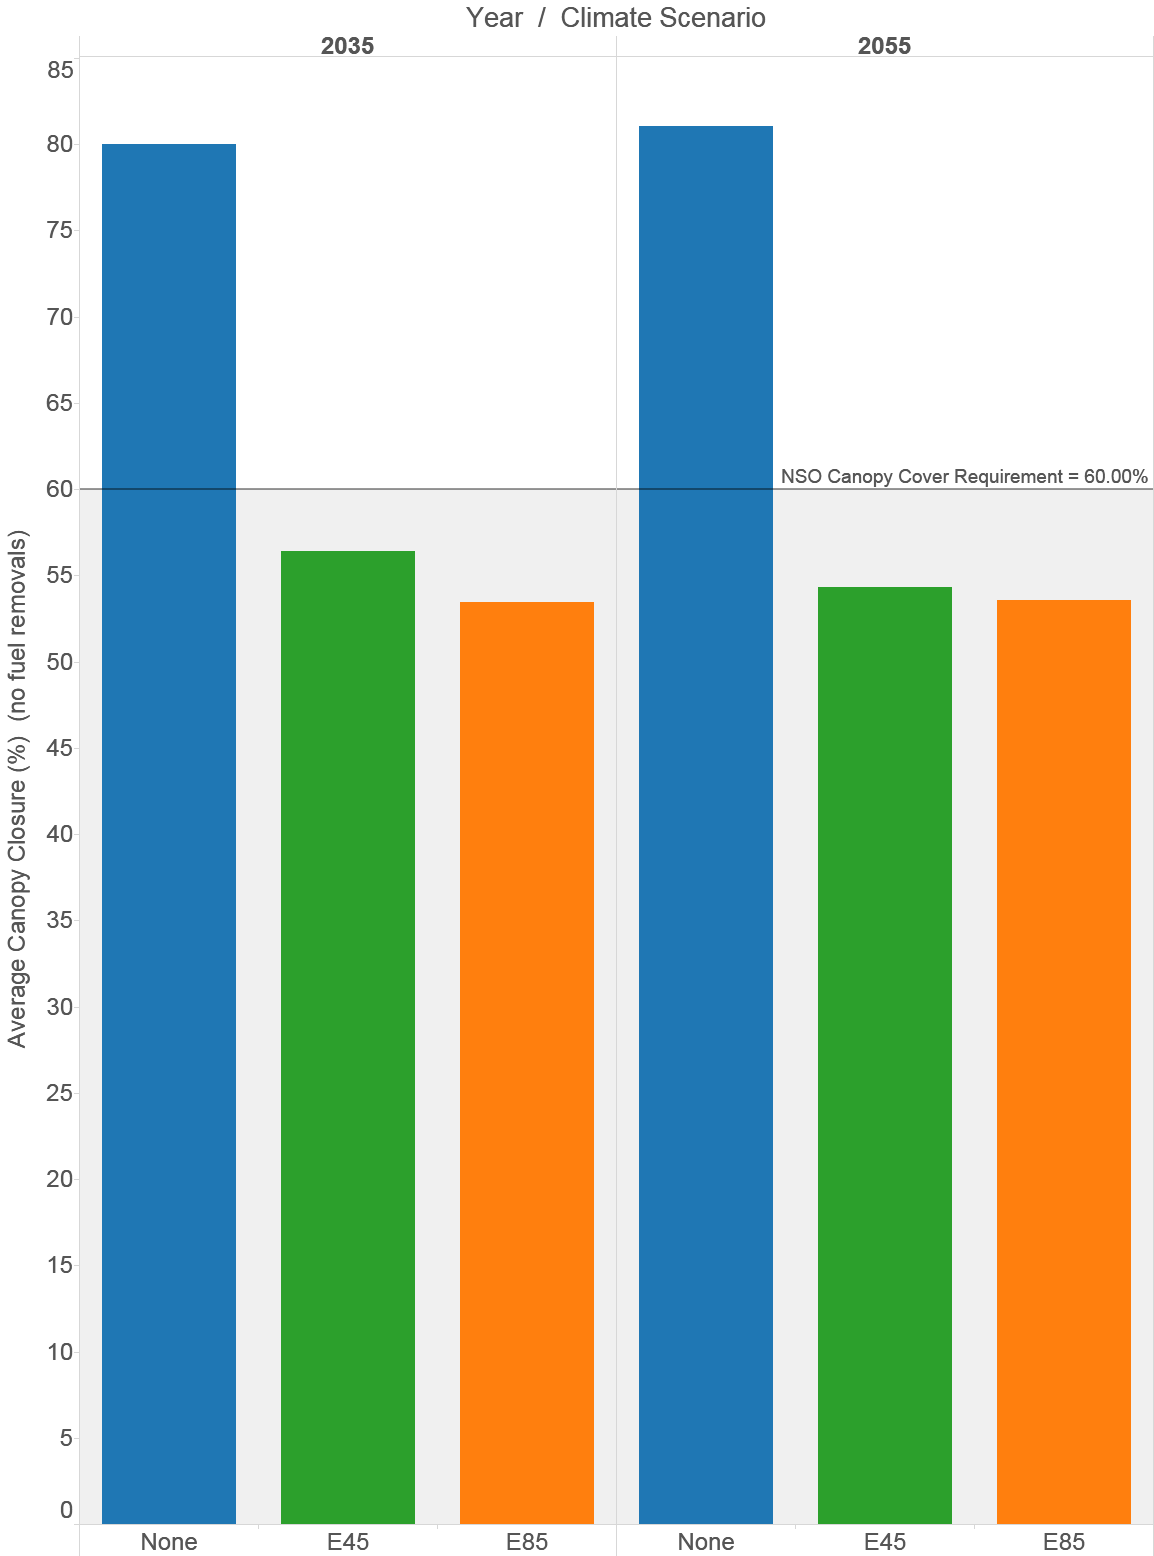
\includegraphics[width=.5\textwidth]{../images/AvgCanopyCover_NoTrtmts}
\caption[Average canopy closure in the Drink Area across climate scenarios]{Average canopy closure for stands in the Drink Area for each climate scenario. Shown are canopy closure values during years 2035 and 2055 (the years in which NSO habitat is measured) when no fuel removals are performed. We see that with increasing climate change severity, canopy closure decreases.}
\label{fig:canopyClosure}
\end{figure}

We also find that the range of achievable values of NSO habitat increases with climate change severity FROM 8 TO LIKE 50 TO LIKE 300.
% BEGIN DISCUSSION
There are two primary drivers for this increase. The first is in the impact of fuel removals on the amount of NSO habitat available. We see in Table \ref{tab:nsoHabDQs} the number of instances in which performing a fuel removal disqualifies a stand from being NSO habitat under each climate change scenario. This happens more than twice as frequently in E45 and E85 than in None. Second, we find that the reduction in fire hazard that results from performing a fuel removal which leads to the disqualification of NSO habitat increases with climate severity. That is, the model is more incentivized to sacrifice NSO habitat in favor of fire hazard reduction. This in turn leads to a reduction in clustering of NSO habitat, further reducing the objective function value (equation \eqref{eqn:eqn:constraintDefOwl}). This data is shown in Figure \ref{fig:nsoHabDQFHEfficacy}, in which we see the reduction in fire hazard as a result of fuel removals that disqualify a stand as NSO habitat. These values increase with climate change severity.

\begin{table}[ht]
\centering
\caption[Frequency of NSO habitat disqualifications across climate scenarios]{Shown here are the number of times for each climate scenario that a fuel removal triggers the disqualification of a stand from being NSO habitat.}
\label{tab:nsoHabDQs}
\begin{tabular}{l|l}
\textbf{Climate change scenario} & \begin{tabular}{@{}l@{}}\textbf{Disqualifications of NSO habitat} \\ \textbf{as a result of fuel removals}\end{tabular} \\ \hline
\textbf{None}                    & 24                                                                               \\
\textbf{Ensemble RCP 4.5}        & 63                                                                               \\
\textbf{Ensemble RCP 8.5}        & 67                                                                              
\end{tabular}
\end{table}

\begin{figure}[ht]
\centering
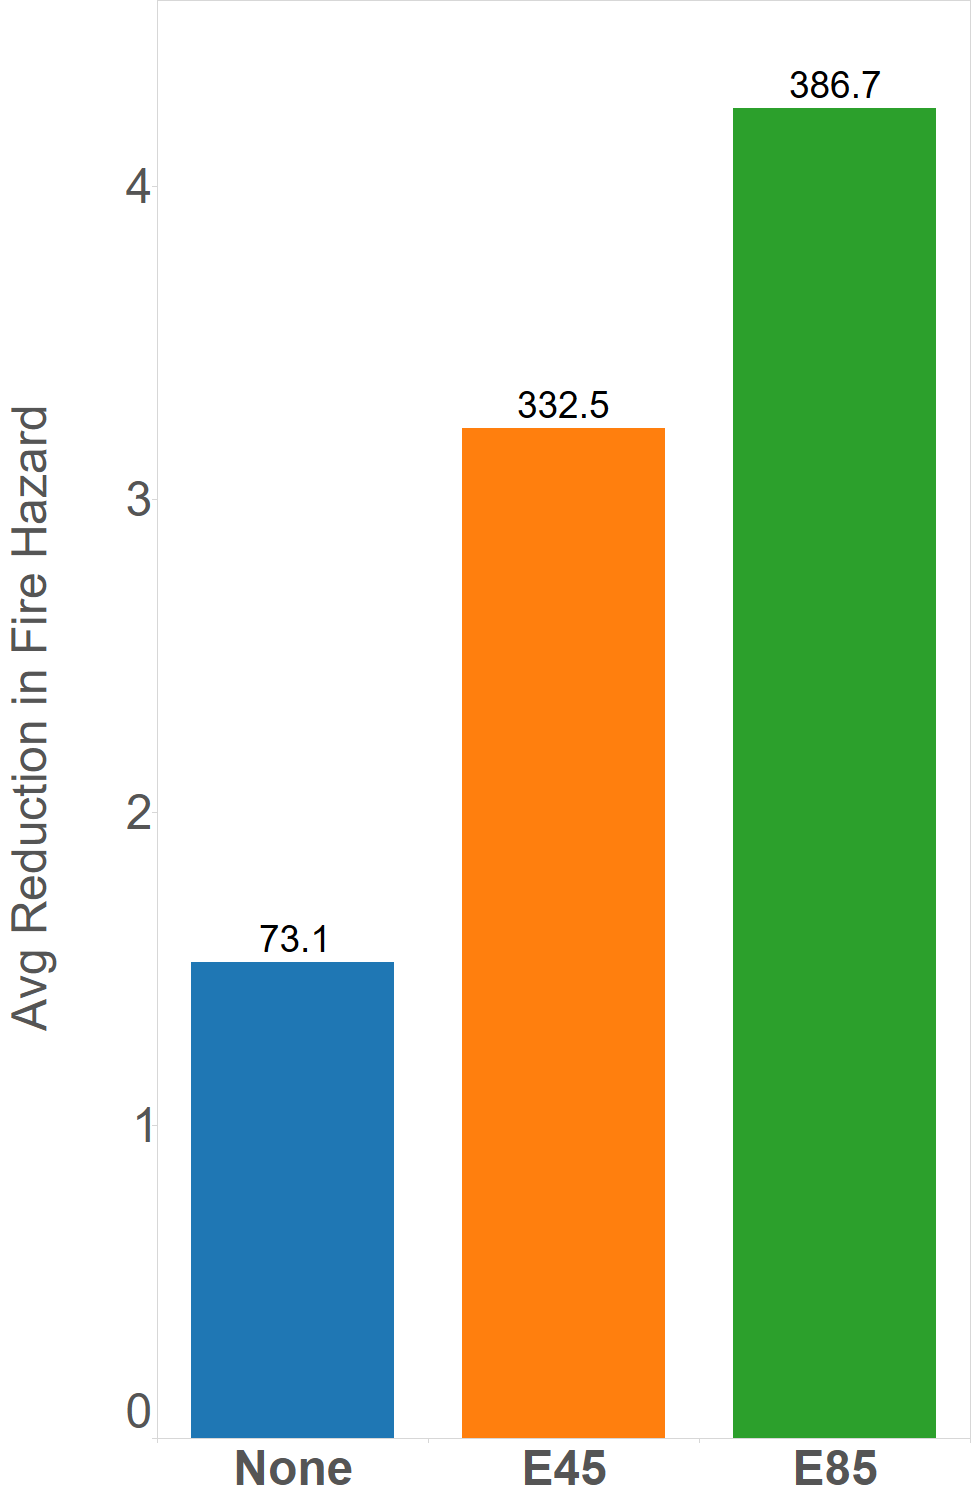
\includegraphics[width=.5\textwidth]{../images/AvgFireHazardEffectivenessForNSODQs}
\caption[Efficacy of fuel removals for NSO habitat disqualification]{Some stands may always be NSO habitat and others may never be NSO habitat, regardless of model decisions. For those stands which vary based on model decisions, we see here the average efficacy of fuel removals which disqualify their being NSO habitat. This value increases with increasing climate change, indicating greater incentive for the model to forgo NSO habitat in favor of fire hazard reduction.}
\label{fig:nsoHabDQFHEfficacy}
\end{figure}
%Could add a figure to show the map of what's NSO hab in a good sol vs a bad sol. Already made this on my work computer. Use it if req'd

We next consider how climate change impacts the joint provision of ecosystem services and the conflict among them.

\subsubsection{Joint provision of ecosystem services}
As we saw for provision of individual ecosystem services, our results show that climate change will have an impact on the joint provision of ecosystem services as well. We observe a decreasing hypervolume with increasing severity of climate change - see Table \ref{tab:hypervols}. A decreasing hypervolume is indicative of more conflict in the system, meaning that climate change is associated with more conflict among the ecosystem services.

\begin{table}[]
\centering
\caption[Hypervolumes of the efficient frontiers]{Hypervolume for each climate change scenario. Hypervolume values increase with increasing severity of climate change.}
\label{tab:hypervols}
\begin{tabular}{lllll}
\multicolumn{2}{l|}{}                                                  & \textbf{None} & \textbf{E45} & \textbf{E85} \\ \hline
\multicolumn{2}{l|}{\textbf{Hypervolume}}                              & 0.876977      & 0.866857     & 0.829541       
\end{tabular}
\end{table}

% Discussion starts here
The difference in hypervolume between None and E45 is approximately 0.01. Recall that a difference of $h$ in hypervolumes equates to a difference of $h^{1/M}$ in each objective. Thus, despite the small size of the difference between $I_{H1}(Z_\text{None})$ and $I_{H1}(Z_\text{E45})$, it signifies an additional achievement in each objective of approximately 21.6\%. The difference is greater between None and E85, approximately 0.05, which represents an additional achievement in each objective of 36.2\%.

% Continues here
From the hypervolumes alone, it is uncertain whether None represents a strictly better frontier than either E45 or E85 or if, despite their smaller hypervolume values, E45 and E85 enclose some region of the objective space that is not enclosed by None. Any such region would extend further into the objective space, representing the presence of solutions for whom greater joint provision of ecosystem services is possible. We use the binary hypervolume indicator $I_{H2}$ to detect the presence and size of these regions. The binary hypervolume values for each pair of frontiers are shown in Table \ref{tab:binaryHypervols}.

% And definitely STOPS here (this is results-- binary hypervol. Add ref to table from prev paragraph to this one)
The binary hypervolume values tend to align with the hypervolume values, with larger values of $I_{H2}(Z_1,Z_2)$ when $I_{H1}(Z_1) > I_{H1}(Z_2)$ and smaller values when $I_{H1}(Z_2) > I_{H1}(Z_1)$. Interestingly, all binary hypervolume values are positive, indicating that no frontier is dominated by any other. This region of the objective space bound only by a frontier $Z_i$ indicates the presence solutions in climate scenario $i$ that achieve greater joint provision of ecosystem services.% than those in the other climate scenarios in this region. 

\begin{table}[]
\centering
\caption[Binary hypervolume values for each pair of climate scenarios]{Binary hypervolumes for each pair of climate scenarios. No values are negative, indicating that no frontiers are dominated by another and that all frontiers uniquely enclose some volume of the objective space.}
\label{tab:binaryHypervols}
\begin{tabular}{ll|l}
\textbf{$Z_1$} & \textbf{$Z_2$} & \textbf{$I_{H2}(Z_1,Z_2)$} \\ \hline
\textbf{None}  & \textbf{E45}   & 0.026154                   \\
\textbf{None}  & \textbf{E85}   & 0.058001                   \\
\textbf{E45}   & \textbf{None}  & 0.016034                   \\
\textbf{E45}   & \textbf{E85}   & 0.045156                   \\
\textbf{E85}   & \textbf{None}  & 0.010565                   \\
\textbf{E85}   & \textbf{E45}   & 0.007841                  
\end{tabular}
\end{table}

To determine the location of these regions and better understand the basis of the change in conflict between climate scenarios, we examine pairwise objective relationships.

\paragraph{Sediment delivery-NSO Habitat}
We observe no clear relationship between climate change severity and the conflict between sediment delivery and NSO habitat; see Figure \ref{fig:pairplotNSOSed}. The figure shows the efficient frontier plotted in the sediment delivery-NSO habitat plane, where each objective has been normalized such that better values are higher and worse values are lower. For instance, in this graph, the point $(1,1)$ represents 0 sediment delivery and maximum NSO habitat. We see similar uniform spreads of solutions for each climate scenario.

\begin{figure}[ht]
\centering
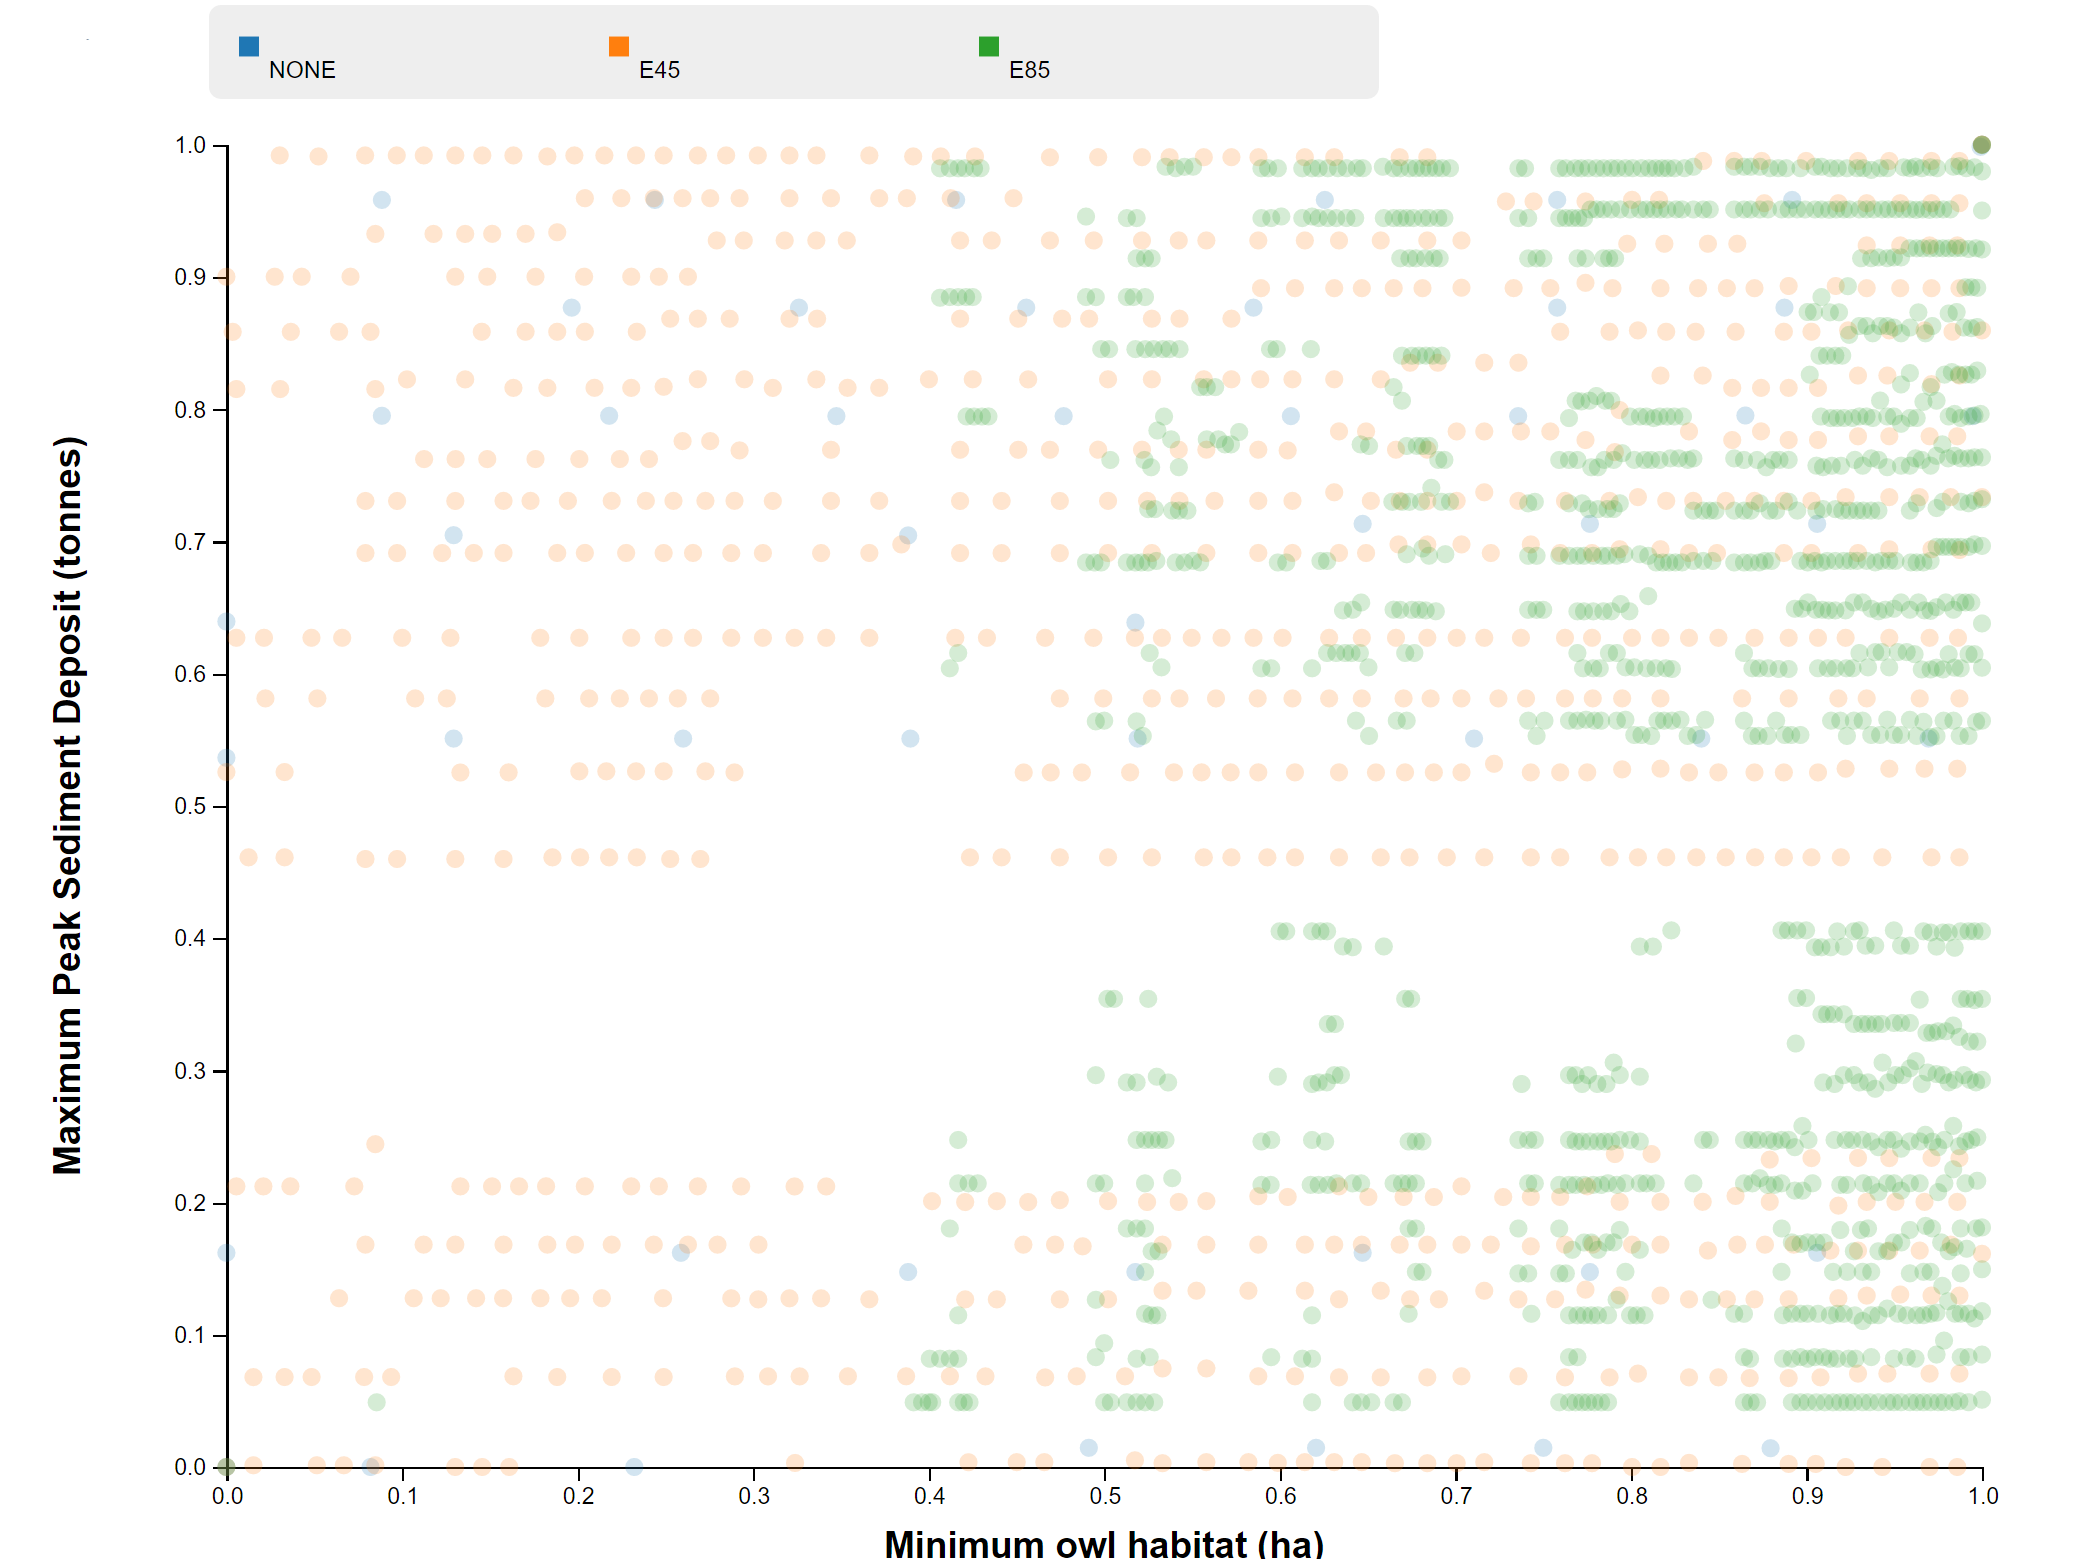
\includegraphics[width=.75\textwidth]{../images/2DSlice_NSO_Sed}
\caption[NSO habitat vs. sediment delivery for all climate scenarios]{NSO habitat versus sediment delivery for all climate scenarios. No obvious conflict pattern exists between the objectives in any climate scenario.}
\label{fig:pairplotNSOSed}
\end{figure}

The values for pairwise conflict also indicate a lack of conflict, as seen in Table \ref{tab:pairConflict-SedNSO}. Values for $C_{ij}$ are all less than $0.25$, with the highest value for the E45 scenario and lower values for E85 and None.

% Discussion starts here
To determine the reason for the variation in $C_{ij}$ by climate scenario, we disassemble the conflict metric into components. A value of $c_{ij,\rho} = 0.5$ indicates the absence of rank correlation, and we find no climate scenario that differs significantly from this value. Lower values of $c_{ij,\rho}$ indicate positive rank correlation, such as in None ($c_{ij,\rho}=0$ for non-conflicting objectives); higher values for $c_{ij,\rho}$ indicate more conflict. $c_{ij,d} \in [0,1]$ represents the average distance of solutions from the sub-dimensional ideal solution. The solutions in the E45 and None scenarios are further away from the sub-dimensional ideal solution than those in E85 leading to larger values of $c_{ij,d}$, but all climate scenarios have on average solutions that are near the mid-point mark of $c_{ij,d} = 0.5$.

\begin{table}[]
\centering
\caption[Sediment-NSO conflict across climate scenarios]{Conflict between sediment delivery and NSO habitat across climate scenarios.}
\label{tab:pairConflict-SedNSO}
\begin{tabular}{l|l|ll}
\textbf{}     & \textbf{$C_{ij}$} & \textbf{$c_{ij,\rho}$} & \textbf{$c_{ij,d}$} \\ \hline
\textbf{None} & 0.19639           & 0.3974                 & 0.4942              \\
\textbf{E45}  & 0.25667           & 0.5194                 & 0.4941              \\
\textbf{E85}  & 0.19284           & 0.5160                 & 0.3737             
\end{tabular}
\end{table}

\paragraph{NSO habitat-fire hazard}
According to the conflict metric proposed here, the conflict between NSO habitat and fire hazard is small for all climate scenarios but appears to decrease with increasing severity of climate change. We find this is due primarily to the increasing density of solutions nearer the sub-dimensional ideal solution in the E45 and E85 scenarios compared to None. See Figure ADDIN2DSLICEFIGURE. Breaking the conflict metric again into components (see Table MAKETHECOMPONENTRYTABLE), we see that the average distance to the ideal decreases with increasing severity of climate change, while the rank correlation again does not differ significantly from $0.5$.

\paragraph{Fire hazard-sediment delivery}
In all climate scenarios, the strongest pairwise conflict is between fire hazard and sediment delivery. This is apparent from both Figure MAKE2DSLICEFIGURE and the conflict metric MAKECOMPONENTTABLE. All rank correlation conflict values $c_{ij,\rho} > 0.95$, indicating strong negative rank correlation. In Figure MAKE2DSlICEFIG we observe a clear void of solutions in all climate change scenarios near the sub-dimensional ideal solution at $(1,1)$, unlike in Figures \ref{fig:pairplotNSOSed} and NSO-FIREFIGURE. We also notice that the None and E45 solutions generally extend beyond the E85 solutions in this plane.

% Now discussion
All fuel removals on watershed stands induce sediment delivery - refer again to Figure (the figure which shows sed deliv per fuel removal) for the average sediment deposit per fuel removal. We can also consider the relative gain from performing these fuel removals. That is, what is the average reduction in fire hazard per tonne of sediment delivered? This is shown in Figure MAKEFIGFhREDUCPERTONNESED. Both of these figures show that increasing climate change severity should increase the conflict between fire hazard and sediment delivery as a result of the increased tradeoff in fire hazard per tonne of sediment delivered. We observe this, however, the conflict metric is not as different between the climate scenarios as we might expect given the results in these figures. This is due to the availability of watershed stands in the E45 and E85 scenarios for whom the sediment contribution is small relative to the total sediment delivered. Examples of solutions taking advantage of these stands are those in Figure 2DFIRESEDSLICE with sediment delivery > 0.9 and fire hazard < 0.7. However, the number of such stands is limited, and to continue to improve fire hazard, stands with larger resulting sediment deposits must be treated. Since the average sediment deposit is higher for the E45 and E85 scenarios, we see the steep drop beyond about 0.8 FH for E85 and 0.9 for E45. Notice, meanwhile, that None is a more gradual descent given the smaller variation in sediment delivery for fuel removals.

\subsection{Discussion}
MOVE A BUNCH OF STUFF FROM ABOVE DOWN HERE